\chapter{团聚}

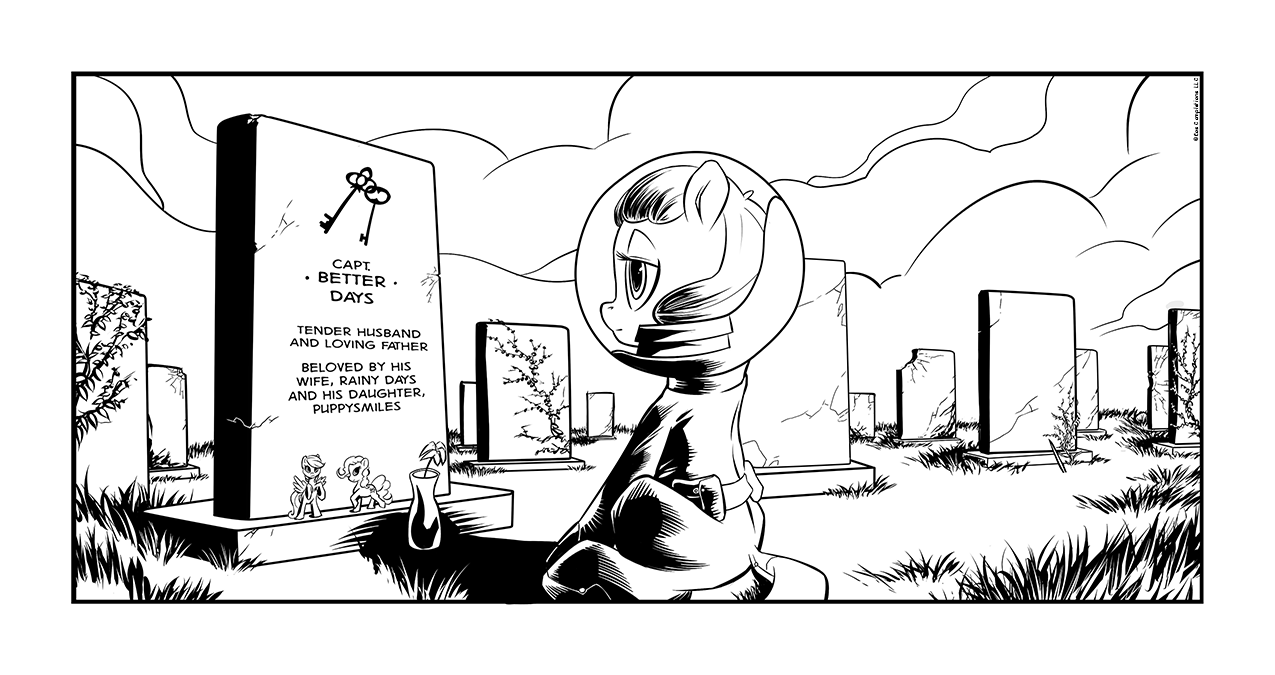
\includegraphics[width=\linewidth]{image16.png}

\begin{intro}
    一个兄弟也不能落下
\end{intro}

「{\rt 我勒个去,伙计们,我简直不敢相信他真的去了!那个羽毛脑袋拿这那个他称之为『步枪』的垃圾烧火棍就那么飞走了!孤狼你如果能听到这个的话,请用那把枪插爆你自己的菊花好么?}」

无线电沉默了一会,然后那个雌驹的声音继续怒骂着。

「{\rt 好吧,朋友们,节目还能继续不是吗?DJ好货现在为您播报52电台。至少在我累趴下之前,因为某个傻蛋把我留下来独自应付一个24小时电台频道!那好,这是我的新规矩,白天我正常广播,晚上只有音乐,因为我又不是什么不老不死不用睡觉的超自然怪物!我也是要吃喝拉撒睡的!如果谁想在晚上找我的话,敲门就是。}」

接下来是一阵翻动纸张的声音。

「{\rt 好吧,不管怎么说,我还是能独自操作这个广播电台的,所以继续把你们的新闻送来就是了,尤其是铁砧镇那边的新闻。说到新闻,纪念碑镇已经被完全摧毁,那里的居民都穿过花椰菜镇到北边避难去了。因此所有要去翡翠海岸的车队,请立刻向北去铁锈庄园,重复一遍,立刻向北去铁锈庄园,不要去花椰菜镇,那里现在太危险了。}」

「{\rt 老娘恨死新闻了,如果有什么消息我会通知你们,如果广播还是音乐那就说明没啥鸟事,这年头没有新闻就是好事。顺便,如果谁见到L.P.请帮我给他脸上来一蹄子。}」


\begin{song}
    小家伙,静静祈祷
    
    Say your prayers, little one,
    
    \medskip

    不要忘记我的孩子
    
    Don't forget, my son,
    
    \medskip

    以及所有小马
    
    To include every pone.
    
    \medskip

    用温暖的怀抱将你包围
    
    Tuck you in, warm within,
    
    \medskip

    洗清所有罪恶
    
    Keep you free from sin,
    
    \medskip

    直到静谧来临。
    
    'til the sandmare she comes
\end{song}

\horizonline

\daytimeplace{13}{4:00 AM}{民族英雄纪念碑公园,52号国道南段}{The Memorial northern picnic area, Big 52 S Branch}

在帕比的远处是一个小小的居民点,是在一尊巨大的雕塑周围堆起来的一堆破烂窝棚。那个雕塑的内容是几位小马士兵共同举着一面小马国旗帜,巨大的雕塑在很远的地方都可以看得清清楚楚。

在来的路上小雌驹见到了好几个难民车队,用马车载着他们不多的家当匆匆向北逃难,她本来想和那些小马聊天,不过那些小马都忽略了帕比,只有几个小孩子挥着蹄子和帕比打招呼。似乎这里的所有小马都在逃亡,放弃了他们赖以生存的土地和家园。

小雌驹现在站在山丘上,一脸疑惑。「呃,声音先生?我们是不是到了爸爸的地方了?」

「{\mt 分析中,定位当前位置:小马国战争英雄纪念碑公园。您的雄性亲属位置:未知。}」

帕比歪着头四处张望,「对哦,我记得这个地方!那个有萍琪派脸的大大路标!」幼驹撒开蹄子飞奔到路边,越过一堆小土丘之后,看到枯黄的草地上到处都是遗弃的营地和生锈的烤肉架。

「这里就是爸爸在的地方!爸爸就在附近!走吧!」

黄色小雌驹飞快地奔向远处,穿过那些低矮的小土丘。即使走了这么远,战争英雄纪念碑白色的碑体依然依稀可见。

穿过这些山丘之后,帕比看到了一棵死掉的树。在记忆中这里曾经是一棵巨大的橡树,但是现在这里只剩下了烧焦的黑色树枝。

这里曾经也是绿树成荫,翠鸟在碧蓝的天空下歌唱……

\emph{「我还要吃苹果派!」}

\emph{「别吃那么多帕比,我们还要去爸爸那里,记得吗,如果你吃得太多又会觉得困了,你不想迷迷糊糊地见爸爸,对吧?」}

\emph{「妈,他一次都没来过,我们去了很多次他都不在!这一次他会在么?」}

\emph{「我……我不知道帕比,不过你可以把漂亮的花留给他呀,他看到的时候会记得你爱着他的,好吗?」}

\emph{一对小雄驹相互追逐着消失在山丘之后,这里的小马都在开心玩耍,吃着午餐,大家都很快乐。}

\emph{「这一次我有更好的东西!你看!」}

\emph{「帕比,这个是你的玩具呀……你真的要把玩具留下么?」}

\emph{「当然!这样爸爸回来的时候就能玩到玩具,他就不会觉得寂寞了!而且,他回家的时候也会帮我把玩具带回来吧。」}

\emph{「……」}

% NOTE: 漏一句

\emph{母女俩在其他小孩子的欢笑声中沉默着。}

\emph{「妈妈?你为什么哭了?「}

绕着这棵巨大的树,小雌驹回忆着之前的时光。她清楚记得春天的时候还在这里野餐。但是现在为什么……大家都去哪里了?记得妈妈说树在冬天叶子会掉光,草也会枯黄,可能现在就是冬天了吧!

小雌驹想着,向记忆之中的地点飞奔过去。

\horizonline

\daytimeplace{13}{6:00 AM}{小马国52烈士陵园,52号国道南段}{Interequestrian 52 War Cemetery, Big 52 S Branch}

这里的墓穴看起来都一模一样,小小的大理石碑上刻着不同的名字,日期,还有一个可爱标记和一段小字。有些石碑是白色,有些是黑色。帕比问妈妈为什么他们颜色不一样的时候,妈妈却叫她安静,不要打搅那些小马的安眠。帕比不喜欢这个回答,因为爸爸是个非常重要的小马,但是却只有一块小小的白色石头。所以她想要带来更多的漂漂花,因为爸爸是最棒的爸爸。

「{\mt 警告,收到求救广播信号,距离:200米,信号辨识完毕:设备009。警告,收到新求救广播信号,距离:200米,信号辨识完毕:设备020。}」

帕比疑惑地歪着头,「啥,新的广播?我希望这一次不是那个一直有小马在喊『救救我们,我们要完蛋了』啥的逗逼信号……」

「{\mt 否定。信号源为和平部 MK VI 防护服。警告,收到新求救广播信号,距离:200米,信号辨识完毕:设备013。}」

雌驹叹了口气:「不是音乐就别烦我啦,我要去看爸爸,或许他已经回来了我们就可以一起去找妈妈了!」帕比说着走向有天角兽雕塑的山坡。

山顶上被矮栅栏包围的是一个烈士公墓,帕比穿过的入口处还有一座高大的坦克雕塑,黄铜牌子上铭记着这里埋葬着的第三装甲师的阵亡官兵。还有一些字写着:因为动力装甲的原因,所以坦克已经不那么常见了。

黄色的小雌驹来过这里可不止一次,所以她对这里的路很熟悉。但是看到这里已经完全沦为一片废墟之后,帕比叹了口气,坐在了一块白色石头前面。

在大理石的表面铭刻着一个可爱标记,还有这么几行字:

\begin{center}
    队长晴空·戴斯

    体贴的丈夫和温柔的父亲
    
    他的爱妻阴雨和女儿快乐帕比敬上
\end{center}

下面的日期已经模糊不清了,不过对于帕比来说没什么意义,因为她早已经来过这里多次。在这块小小的墓碑前,放着一个空瓶子和几个小玩偶。那个瓶子曾经装着鲜花,不过现在里面只剩下了泥水,那些小玩偶依然站在墓碑上看着帕比,两个发霉的小马玩具其中之一是萍琪派,另一个是云宝黛西。

帕比叹了口气:「他从来没回来拿走礼物,为什么他从来不拿我放在这里的东西呢?我觉得他肯定喜欢萍琪派和云宝黛西的。」小雌驹用蹄子碰了碰蓝色的天马玩具,「爸爸好讨厌哦,要是他能经常回家妈妈也不会那么伤心了……」

不过,妈妈也说过很多次,就算爸爸不回家她也不会生气。小雌驹并不明白为什么,不过每一次说到这些妈妈的眼神似乎都不想再说下去,只是让她听话就好。有一天帕比说爸爸不回家自己也不回家,帕比从来没有见过妈妈那么生气地大哭大叫,后来帕比学会不要去问这个问题,或许某天爸爸想起来还爱着他的妈妈就会回家了。

帕比清了清喉咙,然后说:「拿出所有东西。」

「{\mt 警告,物品管理法术每一次只能拿出一样物品,因此打开快速浏览模式,当你检视完成当前物品时,说『下一个』会拿出下一个物品,说『停止』或者『退出』会结束快速游览模式。}」

一个烟灰缸出现在帕比面前,「下一个!」于是另一个烟灰缸\footnote{烟灰缸 (Ashtray):按名称排序,字母A在最靠前的位置}出现了,「下一个!」咻,烟灰缸,「下一个!」烟灰缸,「下一个!」还是烟灰缸……是不是之前提过帕比总是要捡起每一个闪闪发光的东西么?看起来这回要花不少时间。

\horizonline

\daytimeplace{13}{7:00 AM}{小马国52烈士陵园,52号国道南段}{Interequestrian 52 War Cemetery, Big 52 S Branch}

「下一个!」第二十个餐叉收回了帕比包裹里面,然后还滴着水的毛球出现在幼驹面前,「下一……天啊!毛球!」帕比抱起了死去的肉食灵,这个可怜的生物已经没有腿了,只剩下一片翅膀,绿色的粘液从破碎的壳里面流出来,看起来就像是一滩恶心的腐烂物。

「你看起来不是很健康哦,毛球,到底怎么了?」帕比研究着那个死去的生物,想要知道究竟发生了什么,「呃,声音先生,毛球生病了吗?」

「{\mt 否定,毛球已经死亡,并且正在腐烂。}」

帕比皱了皱眉头,她还不太理解那些话的含义,「呃……你是说,她很累么?」

「{\mt 否定,该生物正在变成碎片,正在被自然降解。}」

「什么?」小雌驹警觉地竖起耳朵,「变成碎片?但是毛球不能变成碎片!」她看了看那个尸体,「而且,在我看来好像它还是一整片。」

「{\mt 建议:仔细观察,该生物已经失去三个翅膀和所有的腿,而且因为不良储藏手段正在快速腐烂。}」

「储藏?你是说毛球因为我带着它而变糟么?但是……这太可怕了!」

于是这个没什么自主思考能力的自律智能也劝起了帕比。

「{\mt 肯定,尸体因为你坚持带着它而加快了腐烂进程,推荐您立刻抛弃尸体。}」

帕比很忧伤,「把毛球……留在这里?但是……但是它会寂寞的!这里什么都没有,这里只有……」小雌驹顿了顿,回头看着她父亲的坟墓,「呃……或许爸爸会照顾好它。」小雌驹看起来对这个建议不太感兴趣,虽然看起来这么做没错。

「{\mt 计算,将死亡宠物留给死亡监护人是……错误……错误……请重新思考。}」

「重新啥?你在说什么呢,笨声音,能认真点么。」

「{\mt 再计算,无法找到逻辑,强烈建议寻求其它建议。}」

帕比生气的叫起来:「别说奇怪的话好么,要不然找其他小马来帮我的忙!」小雌驹蹄子按着自己的头盔说:「我说,有时候和你呆在一起真麻烦。」

守望者的金属声音打断了小马和自律智能的争吵,「帕比,你在这里干什么,这里很危险。」

帕比转向声音的方向,黄色的小雌驹看到一个机器精灵飘在那边,不过这一次她没有笑起来,「哦,是你啊,提问者,」

「守望者……」

「随便啦,现在我很烦,回头在找我好么?」

声音迟疑了一下回答道:「可以,但是我现在想警告你,这里不是什么好地方,到处都是……呃……坏蛋,在我走之前你保证赶紧离开这里好么?」

帕比沮丧地哼了一声:「不行,我的毛球生病了,而且声音先生又在发神经!」帕比说着把死掉的肉食灵给机械精灵看。

「哎呦!这东西已经烂掉了!这是啥啊帕比,赶紧扔掉呀!」

「什么?不行!毛球是我最好的宠物和朋友!我喜欢它,它也喜欢我,我们一起冒险这么久了!我不想抛弃它……」幼驹说着撇开了视线,「不过……」

「不过?」守望者追问着,因为帕比抱着尸体不想把话说完。

「不过它病得很重,声音先生说它需要休息……我可以把它放在我爸爸这里,不过好像不太对……因为我还没问他我能不能养宠物……」

「你爸爸?你都知道你爸爸在哪里你还独自在废土上乱逛?」机器的声音听起来有点生气,「到底是哪个不负责任的父亲把自己的孩子……」说到这里,守望者停下了,因为他看到了帕比面前的那块小小石碑。「哦,我的天……还真是……」

幼驹继续说着:「我知道爸爸妈妈说可以,我才能收养宠物……但是……但是……」小雌驹低声哭着,「但是我只是想要个能陪我在一起的朋友!不是一个一直发神经的奇怪声音或者一个来来去去的傻瓜小鸡!毛球从来没有丢下我,一直和我在一起,我们一起玩得很开心,我保护它不被吃宠物妖怪吃掉,而且它从来没有离开过我……」

小雌驹顿了顿,看着机械精灵说:「……现在它生病了,而且腐烂了!声音先生说它之前有更多的翅膀,不过我不太擅长数数,所以我觉得好像他说的没错……我不想把它留在这里,但是我也不想让它因为我而生病……我……我不知道怎么办!」

「啊,那声音先生说什么?」

帕比抹着眼泪,「什么也没说!就是啰里吧嗦的发神经!我想过把它留给爸爸,但是我不知道爸爸是不是喜欢它,爸爸会不会生气……而且,我不知道爸爸什么时候回来这里,因为他从来没有来过这里。虽然妈妈说他爱着我,但是我不知道为什么爸爸一直不见我!」幼驹挥着蹄子,「所以,或许他不会喜欢毛球,毛球也不会开心,但是我不能带着它因为它会腐烂,我觉得腐烂不好……」

守望者纠结着,帕比这番话的沉重感令他一时间不知如何是好。「好吧……或许你可以把毛球给我?把它放在这个机器精灵的货仓里面我来帮你忙?如何?」

帕比歪着头:「你会治好它吗?真的吗!」

「当然,反正它也不会更糟糕了,我看看我能做点什么,不过现在请务必离开这里,这里很危险。」说着,机器精灵旁边打开一个舱门,正好有个可以放肉食灵的空间。

小雌驹看了看这个金属盒子,然后看了看毛球,叹了口气,最后一次抱紧她的宠物,和它低声道别:「别怕,提问者是个漂漂马,等它治好你我们就又可以一起玩了……」在玻璃头盔后面吻别毛球之后,帕比把肉食灵尸体放进机械精灵里面,然后那个舱门关了起来。

「小家伙,别担心她了,她已经去了安全的地方了……现在我们也去安全的地方,好不好?」

小雌驹点了点头,再看了她父亲的坟墓一眼,「百合!」一朵塑料花出现在她面前,她把花朵放在大理石墓碑前,「对不起爸爸,我要走了,下一次我会多等你一会儿,好吗?我会带着妈妈来。」帕比离开了坟墓,转过头面对机器精灵的时候已经带上了她天真的笑容:「好了,我们走!」

「你真是个好孩子,帕比。」

幼驹和机器一起离开烈士陵园,走向纪念碑,那个纪念碑上的小马在常年风化之下已经倒在了地下,正如这里埋葬的士兵一样——在一场没有赢家的愚蠢战争中倒下。

\horizonline

\daytimeplace{13}{7:15 AM}{民族英雄纪念碑,52号国道南段}{The Memorial, Big 52 S Branch}

纪念碑镇已经完全搬空了,这里的居民把所有能带走的都带走了,甚至连松掉的螺栓都拧下来带走了。两个小马骑着狮鹫降落在这里的时候,迎接他们的只有锈迹和灰尘。

「我们到了。」白先生从狮鹫背上跳下来,活动着僵硬的四条腿。「这一路可真远啊。」白苹果的头头扶正他的帽子说:「你们现在可以回太阳城了。」

狮鹫佣兵点了点头,「遵命老大,不过你真的要我们回去吗?」

公马笑了笑,看着身边的另一位小马然后说:「当然,这是家务事,我们只是要你们送我过来,现在没你们的事了。」

看着狮鹫依然不放心的表情,独角兽补充道:「别担心你的酬劳,就算我回不去了,我儿子也会接手公司的。」

带翅的半狮子对其他同伴挥了挥爪子,「好了,你们这群懒翅膀都听到了,走了走了!」于是这些狮鹫都向北边飞去了。

白先生看着那些狮鹫飞走的时候,士官灌木正在把一个沉重的箱子拖进一个用路标之类废铁搭成的小窝棚里面,累得气喘如牛,他抱怨着,「这玩意儿太沉了,白叔叔,你确定我们要拖着这东西走吗?」

「别担心小子,我们就在这里扎营,然后轻装上阵,她不会跑太远。」

「我还是不明白为啥你要自个儿跑这么远,我们大可以叫一大队人马……」

「首先,我们需要尽快来到这里,我们没有那么多空中部队运送士兵和重装备。而且,铁锈庄园出了大价钱雇我们的佣兵队,有钱为啥不去赚。另外,我们又不是来战野牛帮的,我们只是跑过来接小孩的。」

灌木叹了口气,「难道没有人和你说你是个怪胎么,我知道她把我们从火坑里面拉出来的,但是你已经给她报酬了,不管怎么说我觉得这个任务纯属自杀。」公马犹豫了一下,然后又问:「或许还有啥内情?」

白苹果的头头正拿着一个望远镜看着附近的山头,「根据我之前打探的消息,不管那幼驹跑哪儿去,似乎哪里都会变得……嗯……更好,那个『幽灵』肯定是某种福星啥的,我这次要亲眼看看那小雌驹有多大能耐……」

灌木不相信地摆了摆蹄子,「你下这个结论是基于……」

「直觉。」

狙击手以蹄覆面,「我们大老远跑过来找个幽灵是因为你的一个第六感么,为啥我要跟你来?」

白先生笑了,「因为我是你叔叔,而且你欠了我一屁股债。」

「我恨我自己……」灌木刨着地。

白色的独角兽举起蹄子示意安静,「安静,有谁来了,拿枪。」

从他们的狙击地点,两个小马可以清楚看到有谁正在走向小镇,那个旅者满身尘土,厚实的纱巾挡住了她的脸,遮住了她的容貌,在脖子上挂着一长串羽毛和各种小物件装饰的项链。

灌木放下了步枪松了口气,「哎,就是个先知……而已,萨满跑到离沙漠这么远的地方做什么?」

白先生放下枪走出窝棚,「我们马上就知道了。」独角兽说着奔向那个新来的小马。

「喂,叫你呢!这里什么都没有,路南边很危险,你赶紧回去吧。」

戴面纱的小马站住了看着白先生,然后脱下了自己的头纱,露出一个老独角兽雌驹的脸,「你们已经来了……非常好,我们在这里等待其他小马到来吧。」

\horizonline

\daytimeplace{13}{7:30 AM}{纪念碑镇外,52号国道南段}{The Memorial outskirts, Big 52 S Branch}

「对了帕比,你还没跟我说过你鬃毛里面的蓝条是怎么回事,怎么来的?」机器精灵漂浮在帕比身边,他们俩慢慢地走向纪念碑镇,烈士陵园的大门就在他们身后。

「啊,就是在太阳城,蓝音欺负我的时候,我记得不太清楚,不过好像是我睡着了,醒来以后我的鬃毛就变得这么时髦了。」

「这样啊……你睡着了再醒来鬃毛就变了?蓝先生和你说啥了?」

帕比叹了口气,「我和你说过了呀,他说我是个机器马,不过我好好教训了他,而且那都是过去的事了,现在我们已经是好朋友了。」

「啥啥啥?你们是朋友?你不是用一个魔能脉冲弹头炸死他了么。」

帕比咯咯笑着,「当然不是,笨笨提问者,他不是坏机器,不过是一个傻瓜男生!第二次见面的时候怕音帮我教训了他,他和我道歉了,虽然他嘴巴有点毒不过我还是把他当做好朋友!」

「怕什么?」守望者的声音听起来有些担心了。

帕比戳了戳头盔,「你知道的,怕音,住在我脑袋里面说奇怪事情但是又酷酷的坏女孩。」

在一阵长长的沉默之后,机器精灵问:「你是说声音先生么?」

「当然不是,声音先生有点无聊而且说些不明觉厉的话,但是怕音不一样,虽然有点可怕但是酷酷的,她超级厉害的,可以砸烂铁门打飞坏机器。」

机器的喇叭里传来一声惊叹:「哦!我懂了,是你的想象朋友是么?」

帕比歪着头,有点疑惑的说:「她看起来不那么香香?不过好像也没错……」

「好孩子,你总是……」

轰隆!

守望者就在帕比面前消失在一团火球之中。

小雌驹后退了几步,想要搞清楚发生了什么事情。然后她注意到远处有一个巨大的金属物体正在缓缓向她驶来,她马上就明白那是什么了。

「哼,坏机器……」

\horizonline

\daytimeplace{13}{8:00 AM}{民族英雄纪念碑,52号国道南段}{The Memorial, Big 52 S Branch}

白先生坐在窝棚里面的一张桌子后面,而灌木正在一边煮着燕麦。

「长耳,你说的那些小马什么时候会来?」

雌驹耸了耸肩,目视着窗外远处灰暗的天空,「我们明天晚上之前要出发,将会有很多小马,很多腥风血雨……」

灌木转向先知:「老巫婆,我们不是来打仗的,我们只是来接那个幼驹回闹市区,我才不管你那什么疯狂的『预言』。」

白先生对他侄子挥了挥蹄子示意他安静,「你做你的饭,我负责交谈,我想我们早就说好了。」然后他继续问着那母马:「那么,你看到了什么?」

长耳闭上了眼睛,「在梦中我看到火焰从南方燃起,吞没了沿途所有小镇,在熊熊烈焰之中一个粉色的身影在挣扎着,火焰在她穿过的时候似乎熄灭了一些,但是在她离开之后,火焰继续向北边肆虐,而那个身影则在道路的尽头变为黑暗。」

白先生皱起了眉头,「变成黑暗?那是什么意思?」

「一个黑色的波纹在火焰之后形成,并且摧毁了所有东西。」母马叹了口气,当黑色的波纹熄灭火焰之后,整条道路都归于虚无,成为废弃的荒野。」

「好吧,正如我之前的不详预感一样,」灌木叫了起来,「我们赶紧收拾东西回闹市区吧!」

白色独角兽叹了口气,不管他的侄子继续问道:「那么,我们来这里能做什么?」

长耳的视线从窗外回到独角兽身上。「为了阻止火焰毁灭一切,然后在粉色幽影到达道路尽头之前阻止她。」

「粉色幽影?你说啥,我好像觉得你是不是在说那个孤狼说的小小幽灵?」

忽然一声巨响打断了白先生的话,他看着窗外却看不到任何爆炸。

「是火炮?」

爆炸声听起来有点距离,大概在几公里之外。不过白苹果的老大走到外面的时候,却没有任何声音了,不过不知道是不是幻觉,另一只小马出现在远处,身穿一件破烂的披风,头上还带着一顶大帽子。

独角兽喊了起来:「喂,你!这里很危险,回花椰菜镇去!」不过在看清楚来者之后,白先生的声音变了。

「你这个老木乃伊……」

融金微笑着走进白先生,「什么风把你吹这里来了老白,我觉得我最不可能在这里碰见的就是你了,你在这个前哨站做什么?这里有做生意的对象?」

独角兽皱起眉头,「老家伙,我可没打算抢你的工作,我们只是在……侦察野牛帮的动向。」他说到这里顿了一下,观察着尸鬼的表情,「那么你在这战火纷飞的地方做啥,这里有珍宝么?」

百年老尸哼了一声,用嘶哑的声音说:「差不多,应该说我不小心送走一个危险物品,所以我打算弥补之前的过错。」

「从来没听过你这个老混蛋还有吃后悔药的时候,怎么了?年纪大了?」

让白先生惊奇的是,老木乃伊没有反驳,只是看着南方。「你说的没错,平时我可不会关心一个幼驹的死活,现在我却去要救一个小鬼。」

白先生的表情慢慢地从惊讶变为微笑。「欢迎加入俱乐部,进来吧,里面不但有燕麦还有美女。」

\horizonline

\daytimeplace{13}{7:45 AM}{民族英雄纪念碑南广场,52号国道南段}{The Memorial southern picnic area, Big 52 S Branch}

帕比冲向那个巨大的机器,而发光的「命运之石」就漂浮在她身边,「你这个坏机器,不准欺负我朋友!」

而帕比冲向的目标,则是一辆锈迹斑斑的老式坦克,不过即使有接近三个世纪的寿命,这辆坦克依然状态良好,一只有刺猬一样鬃毛的小马正坐在车长的位置看着冲向他们的小雌驹。

「肏他妈的命令,为啥我们要在这里蹲着,我们有坦克好不好,坦克!有这宝贝儿我们可以碾平那些原始马。」

「灰质,那黄色东西正朝我们跑过来,不如来点移动靶射击练习?」那个舱口的小马大笑着,回到坦克里面关上舱门。坦克的炮塔开始转向正在跑过来的小马。

在坦克中,那个刺头正疯狂的笑着,「来啊小家伙!」

「等等!」一个剃光头的雌驹用蹄子戳了炮手的屁股,「我们玩点别的!我要玩玩这个!」

「闭嘴,傻……」那个公马正准备把那个多管闲事的雌驹骂个狗血淋头,但是却看到了她蹄子指着的那个红色按钮。「对哦!我也想试试看,让我们用火箭把它炸到月亮上去!」

「你们俩傻逼能不能少说话多开炮?」陆马驾驶员发火了。

炮手笑着:「伙计,你真是个暴脾气,灰质,看这个!」

这个时候,帕比刚刚跑了一半,她可以清楚地看到那个坏机器有一个方方正正的身体,还有个圆脑袋和长长长长的鼻子……想起来了!这个不是坏机器,是马车!是那些有大茶壶的车子!

小雌驹停了下来,好吧……这东西应该不是坏机器,因为车子一般都会有小马在上面,不过她现在看不到上面有小马,而且它还打坏了提问者的机器,这绝对是坏机器干的事情,所以帕比有点不确定这东西到底是坏机器还是车子,她在考虑是不是要去问问看。

这个时候,坦克炮塔上飞出一道白烟,一发火箭弹射了出来,朝帕比飞去,看起来就像个可笑的大号烟花。

「呦呵!好厉害!烟火耶!」

轰隆!

火箭弹打中了小雌驹身后,把小雌驹炸飞了出去,然后一个倒栽葱摔倒在坦克面前。帕比的头盔都碎了,防护服上也都是破洞。粉红色的迷雾从防护服上的破洞喷出来,环绕在帕比身边。

「好吧,这绝对是坏机器……」帕比慢慢站起身,瞪着在她面前的那个巨大钢铁怪物。在粉红色的迷雾之中,没有头盔的帕比面容已经模糊不清,只有两只发着粉色光芒的双眸清晰可辨。

「黄色的玩意儿,尝尝这个!」刺头狂笑着,但是那个雌驹又戳了他一下。

「又怎么了臭婊子?」

「喂,我说,那东西又站起来了……」

「怎么回事?灰质,碾碎它!」

不管怎么说,废土上很多奇妙的东西,当然也包括被火箭弹上脸还能活蹦乱跳的东西,不过那些强盗觉得被坦克的履带碾过绝对能搞定一切。

于是坦克开始缓缓向前,对准小雌驹开了过去,不过帕比也同样冲向坦克,并且在两条履带碰到她之间敏捷的蹦了起来,用蹄子抓着前装甲板跳上了炮塔。

「那东西上坦克了!好运姐,出去打爆它!」驾驶员忽然一个急刹车想把那东西甩下去,可惜帕比抓得紧紧的,而炮手却猝不及防一头撞上瞄准仪昏了过去。

「别担心,看我的!」雌驹用魔法飘着一把冲锋枪打开舱门,发现在她面前就是被一团粉云包围着的小雌驹。「拜拜,怪物!」

帕比听到面前好像传来有谁说话的声音,但是她转过头只看到个小马形状的东西,但是马上就挨了一梭子子弹,打碎了刚刚自动维修好的头盔。

「坏机器,别闹了!」

帕比这一次真的生气了,她跳到了坦克顶上,但是坦克的舱门立刻紧紧关上了。

「你觉得你能把我关在外面吗?我可是快乐帕比,我想去哪儿就去哪儿!」

幼驹举起石头,在炮塔上寻找着可以砸烂的东西,不过都是各种铁块,哦,一个玻璃镜子,……咣当……铁块,铁块,哦,天线,……叮……叮……叮……,还有一个大盒子?「好了,坏机器,打屁股时间到了!」帕比很喜欢怕音说的这句话,听起来坏得有范儿!

而在坦克里面,好运姐正在因为吸入粉雾而大口吐血,额头上肿着大包的炮手还没有醒过来,而驾驶员灰质正在在蹄忙嘴乱的衔着一瓶治疗药水喂给重伤的雌驹。大家都忙得不可开交,而没有注意到那个幼驹正在坦克顶上用石头敲着坦克的火箭发射器。

这差不多是白先生听到那声巨响的时间。

\horizonline

\daytimeplace{13}{9:00 AM}{小马国烈士陵园,52号国道南段}{Interequestrian 52 War Cemetery, Big 52 S Branch}

三个小小的身影在坟墓之间沉默地站了起来。它们全穿着MK VI防护服,就像帕比那件,不过里面不是幼驹,而是腐烂到皮包骨的僵尸。在它们黑洞洞的眼眶之中看不出一丝智慧的光芒,只燃烧着一团粉色的火焰。它们慢慢地跟着地面上小小的蹄印,就像是追随着猎物的猎犬一样,慢慢地向南方走去。


~\vfill

\begin{note}
    升级 (Lv 15) 

    新技能解锁:卧倒!——怎么回事,我绝对打中她了!

    你对爆炸伤害的抗性提高25点,你可以开心地玩火箭跳了。
\end{note}


